\documentclass[a4paper]{article}
\usepackage{latexsym,amssymb,amsmath,amsbsy,amsopn,amstext,xcolor,multicol}
\usepackage{ctex,hyperref,graphicx,wrapfig,fancybox,listings}
\usepackage{pgf,pgfarrows,pgfnodes,pgfautomata,pgfheaps,pgfshade}
\usepackage[top=1in, bottom=1in, left=1.25in, right=1.25in]{geometry}
\graphicspath{{pic/}}
\title{\bf Few-Shot Learning}
\date{2018.6}
\author{翁家翌~2016011446}
\begin{document}
\kaishu
\ttfamily
\maketitle
\tableofcontents
%\newpage
\section{Basic Idea}

在课堂上,崔老师提到对于Few-Shot Learning\cite{fewshot}的一些看法,他指出人脑的学习速度会随着知识量的增加而加快,而现有的网络结构(如AlexNet\cite{alexnet}、VGG\cite{vgg}、ResNet\cite{resnet}等等)都是由数据驱动学习出来的,与人类学习方式不符合,因此提出了这个大作业。

顺着这个思路,我们组继续想下去:

首先,学习的过程对于一个人而言是十分重要的,他会从这个过程中学习到一些学习的方法,而这个学习学习的过程(Meta Learning\cite{maml})也被广泛运用于许多神经网络的任务中,来更好地增加泛化能力。

其次,对于该任务而言,我们有的是一个在ImageNet\cite{imagenet}上pretrain好的AlexNet\cite{alexnet}模型,它对于图像的特征提取已经有了很强的能力,只不过没有对新类别的分类参数。考虑到图像的特征提取对于每个神经网络模型都是通用的,因此我们只决定修改最后一层的分类器。

如果只是简单的修改最后一层,将$[4096,1000]$的分类器改成$[4096,50]$,那和fine-tune没区别,并且也不符合人类学习的方式。因此我们考虑,这些参数是否能够被学习出来,这样一来也能够具有更好的泛化能力。

并且,一个类别中的图片总是对全连接层之前的某些激活节点产生很强烈的响应,举个例子,如果图像是一辆车,那么表示门、窗户、轮子的这些激活节点会产生强烈响应;如果在产生对车的预测概率时候,把门、窗户、轮子的激活节点对应的权重增加,那么是会有益于对车的分类准确性的。因此可以猜想,一张图经过神经网络得到的特征$a_y$,对应某个类别$c$的权重 $w_{c,y}$,如果$a_y\cdot w_{c,y}$足够大,那么分类效果越好。更抽象一点,权重$w$与激活节点$a$是存在某种对应关系的。

因此我们实现了这个方法,实验结果表明它比fine-tune的CNN效果会好一些。为什么好不太多呢?我觉得是数据集之间有overlap,Caltech256\cite{caltech256}其实和ImageNet的Data Distribution挺接近的,因此才会导致baseline太高,而传统的Few-Shot Learning任务定义是新数据集与原数据集完全没有overlap。我个人觉得在Caltech256上面做这个实验不太具有说服力。

\section{Algorithm}

算法的核心思想是学习一个映射函数$\phi:a_y\to w_{c,y}$,根据每个类别中激活函数的统计值来学习这个映射关系。

整个forward的流程如下:

\begin{enumerate}
	\item 使用pretrained AlexNet对训练集图像提取特征;
	\item 对于每个类别,将其所属的图像的activation map取平均,作为这个类别的activation map $\overline{a}_y$;
	\item 使用训练好的映射函数$\phi$(大小为$[4096,4096]$)得出当前最后一层的权重$w_{c,y}$;
	\item 使用该权重(大小为$[4096,50]$)对图像进行最后的预测;
\end{enumerate}

理论上$\phi$能够在ImageNet数据集上直接学出来,然而助教说不让用,并且我们使用的是PyTorch而不是TensorFlow,无法直接使用feature.npy文件,故而只在给出的图片中训出$\phi$的参数。我相信如果加入ImageNet的部分数据,这种方法能够有更出色的表现。

\section{Result}

\begin{figure}[htp]
\centering
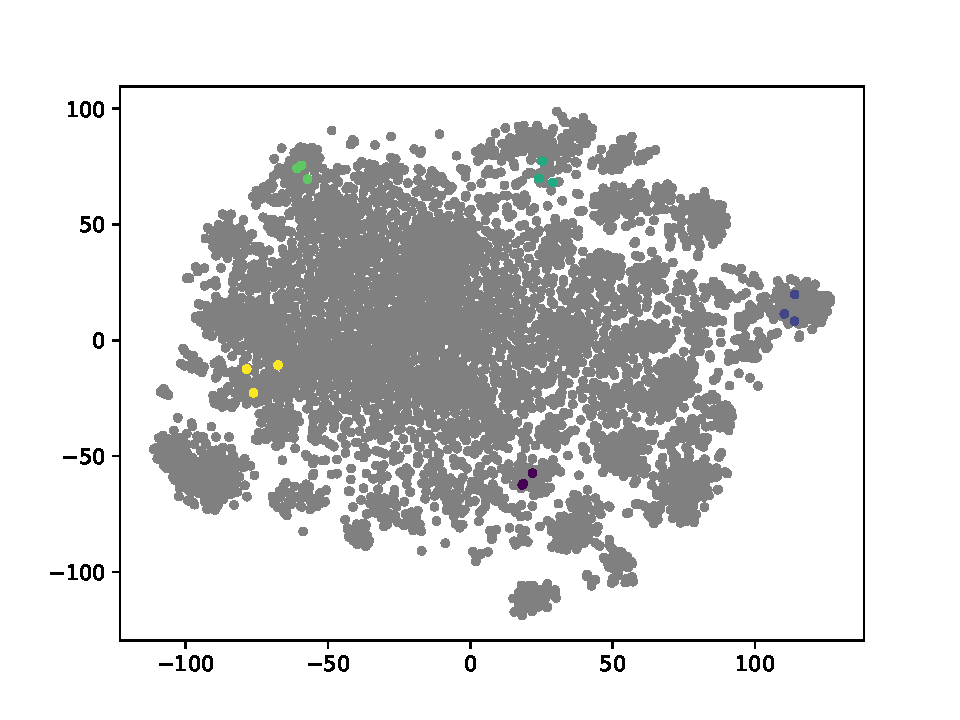
\includegraphics[width=0.7\linewidth]{tsnepca.pdf}
\caption{使用t-SNE\cite{tsne}对测试数据的特征进行可视化,图中灰色的点为测试集,非灰色的点为训练集中带label的图片,相同颜色代表相同类别。}
\label{tsne}
\end{figure}

我们采用了t-SNE\cite{tsne}对测试集数据提特征之后进行可视化,如图\ref{tsne}所示,可以直观地看出,相同的类别在特征空间中的距离十分近。因此猜想最后一层的线性分类器理论上应该有能力将这些特征分类。为了验证这个猜想,我们拿这些500张带label的数据来训练CNN的最后一层分类器,发现能够很快的overfit,因此得出结论:在数据规模不大的时候,单层线性分类器理论上是有能力达到100\%的分类准确率的。这个结论是我们实现方法的一个有力支撑。

\begin{table}
\begin{center}
\begin{tabular}{c|ccc}
	Method & One-shot & Three-shot & Five-shot\\
	\hline
	Nearest Nerghbour & \textcolor{red}{44.0\%} & 56.4\% & 59.6\%\\
	Fine-tune CNN & 37.2\% & 54.8\% & 64.4\% \\
	Our Result & 42.4\% & \textcolor{red}{59.6\%} & \textcolor{red}{67.6\%}
\end{tabular}
\end{center}
\caption{实验结果}
\label{result}
\end{table}

表\ref{result}是实验结果的对比数据表格。从训练图片数量对结果的影响趋势来看,训练图片越多,准确率越高。因此我们最终提交的模型是用10张图训练,不加任何测试集,训练100个epoch,每30次之后learning rate降低至原来的0.1倍,初始的learning rate设置成$10^{-4}$。

我们随机在测试集中选了一部分图片进行标注,结果显示我们的最终准确率大约在$70\%$左右。

\section{Contribution}
在本次大作业中,我担任组长,负责统筹规划任务分配,check进度,以及模型的训练与测试,和baseline的代码编写。我们比较了fine-tune baseline和nearest neighbour in cosine distance两种方法,这两部分的代码以及整体的代码架构都是我写的。以及在代码文件夹下面还有一些其他文件,比如:
\begin{itemize}
	\item[merge.py] 模型ensamble所用;
	\item[xgb.py] XGBoost\cite{xgboost}对于该任务的表现,只有57\%左右的准确率,因此不是很适合该任务;
	\item[tsne.py] 使用AlexNet提取测试集图片的feature之后将其可视化到二维平面上;
\end{itemize}
以上代码均由我完成。

高天宇和杨帆主要负责核心算法的实现、数据处理、参数调整、PPT制作和最后的展示。还有一位同学胡钧,至今没有联系上,因此实际上我们组只有三个人。
\bibliography{ref.bib}{}
\bibliographystyle{plain}
\end{document}
